\chapter{Súčasný stav}

\tab[5 mm] V tejto časti práce sa budeme venovať prehľadu súčasného stavu problematiky ovládania pomocou biosignálov, so zameraním na domáce a zahraničné výskumy a implementácie, a ktoré boli počas robenia tejto diplomovej práce skúmané, poprípade uvažované. Pozrieme sa napríklad na vývoj elektroencefalografu (EEG signálov),  elektromyografického (EMG signálov), elektrokardiografického (ECG signálov) a elektrodermálneho (EDA signálov), na Brain-Computer Interface (BCI) technológie ako bitalino, neuralink, asistenčné technológie ako prístroj na ovládanie počítača pomocou očí (toby), úst, asistenčné technológie pre nevidiacich. V tejto kapitole sa budú opisovať rôzne výhody a navýhody daných technológii, poprípade ich riziká.


\section{História}
\tab[5 mm] Táto podkapitola poskytuje prehľad o histórii EEG, zdôrazňujúc prínosy a vývoj od jeho počiatkov, ktoré boli neoddeliteľne spojené s prácou Hansa Bergera.
\subsection{Prvé Kroky: Objav Elektrických Aktivít v Mozgu}
\tab[5 mm] V roku 1924 dosiahol Hans Berger[4*] kľúčový milník, keď prvýkrát zaznamenal elektrické aktivity v ľudskom mozgu prostredníctvom elektroencefalografu(EEG). Tento objav znamenal začiatok elektroencefalografie a poskytol nový pohľad na štúdium mozgovej činnosti.\\
\subsection{Kontinuálny Vývoj EEG Technológie}
\tab[5 mm] S postupujúcim časom sa EEG technológia neustále zdokonalovala. Výskumy a experimenty Hansa Bergera a jeho nasledovníkov pomohli vytvoriť sofistikované EEG prístroje, ktoré umožňujú detailnejšie sledovanie mozgovej aktivity.
\subsection{Prínosy Pre Medicínu a Výskum}

\tab[5 mm] Hans Bergerov výskum a jeho vynálezy v oblasti EEG mali významný vplyv na medicínsku diagnostiku a výskum mozgovej činnosti. EEG sa stal dôležitým nástrojom pri identifikácii neurologických porúch a štúdiu rôznych stavov mozgu.

\subsection{Nadväzujúci Výskum a Vývoj}
\tab[5 mm] Článok taktiež pripomína, že po Bergerových počiatkoch nasledovalo mnoho ďalších výskumníkov, ktorí prispeli k ďalšiemu rozvoju a porozumeniu EEG. Ich prínosy viedli k rôznym aplikáciám, vrátane vývoja moderných Brain-Computer Interface (BCI) technológií.

\section{Domáce Prístupy}
\subsection{Popis problému}
\tab[5 mm] V kontexte Slovenska je stále vzrastajúci záujem o výskum a aplikácie Brain-Computer Interface (BCI). Práce, ako napríklad [3* - RIADENIE MOBILNÉHO ROBOTA POMOCOU EEG SIGNÁLOV MOZGU DIPLOMOVÁ PRÁCA], ďalšia praca na túto tému [5* - SNÍMANIE A SPRACOVANIE EEG SIGNÁLOV MOZGU PRE ÚČELY VYUŽITIA V SYSTÉMOCH HMI DIPLOMOVÁ PRÁCA], prispievajú k rozvoju poznatkov v oblasti BCI a jeho aplikácií v domácom prostredí.
 
\tab[5 mm] Obe práce sa zaoberajú konkrétnymi aspektmi vývoja a implementácie BCI technológií pre lokalizované potreby, V týchto diplomových prácach sa venovali problematike elektroencefalografie (EEG) a jej aplikáciám.

\section{popis technológií}
\subsection{Elektroencefalograf (EEG)}
\tab[5 mm] Elektroencefalograf (EEG) predstavuje nástroj navrhnutý na zaznamenávanie elektrických aktivít v mozgu. Tieto elektrické signály, generované komunikáciou medzi mozgovými neurónmi, sú zachytávané sériou malých kovových diskov, nazývaných elektrody, umiestnených na povrchu hlavy. Následne sú tieto slabé signály zosilnené pomocou preampfikátora a zaznamenávané elektronickým záznamovým systémom. EEG umožňuje sledovať charakteristické vlny mozgovej aktivity, ktoré sú následne využívané v oblasti neurologie, psychiatrie, a výskumu mozgovej činnosti. Jeho neinvazívna povaha a schopnosť poskytovať detailný pohľad na stav mozgu robia z EEG významný nástroj pre diagnostiku, monitorovanie a vedecký výskum. Na obrázku nižšie vidieť záznam z elektroencefalografu.\\
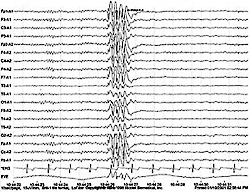
\includegraphics[width=1.0\textwidth]{images/eeg.jpg}\\
\tab[5 mm] Aby elektroencefalograf (EEG) mohol správne fungovať musíme poznať základnú topológiu ľudského mozgu a aj jeho základné funkcie aby sme mohli elektroencefalograf (EEG), Ľudský mozog, zložený z neurónov, predstavuje komplexný neuroanatomický systém, ktorý je charakterizovaný rôznymi stupňami vzájomnej prepojenosti neurónov. V tomto zmysle tvorí kôra mozgu, čo je najvonkajšia vrstva mozgového tkaniva, významnú časť tohto neuroarchitektonického usporiadania. Konkrétne, kôra mozgu obýva približne 70\% neurónovej populácie v ľudskom mozgu[3*]. 

\tab[5 mm] Elektrický signály medzi bunkami ľudského mozgu (neurónov) vzniká v dôsledku ich polarizácie, čo je zachytávané ako elektroencefalografické (EEG) signál. Tieto aktivity môžeme merať aj na povrchu, signál je však veľmi slabí a to na úrovni desiatok mikrovoltov. Hlavnými zdrojmi elektrickej aktivity mozgu sú akčné potenciály a postsynaptické potenciály excitácie a inhibície (EPSP a IPSP)[3*].

\tab[5 mm] Na kôre mozgu sa vyskytujú akčné potenciály a hromadné excitácie postsynaptických potenciálov , čo je zásadným faktorom synchronizovanej aktivity EEG. Synchronizácia výbojov talamických jadier závisí na zmene ich membránového potenciálu prostredníctvom informácií z EPSP, čím sa aktivujú napäťové Ca2+ kanály a vytvára sa cyklus vedúci k akčnému potenciálu talamických neurónov[3*].

\tab[5 mm] Následne nasleduje hyperpolarizácia membrány, ktorá je obnovená prúdom draslíka. Cholinergné vstupy z mozgového kmeňa a predného mozgu udržiavajú membránový potenciál talamických jadier, umožňujúc prenos senzorických informácií do mozgovej kôry v aktívnom stave[3*].

\tab[5 mm] Ľudský mozog, s obsahom 86 miliárd neurónových buniek, zahŕňa viacvrstvovú pavučinu neurónov a rozsiahle množstvo gliových buniek, ktoré stabilizujú chemické prostredie a regulujú a chránia neuróny. Mozgová kôra, ktorá predstavuje približne 70\% všetkých neurónov mozgu, je rozdelená na štyri hlavné časti: čelový lalok, temenný lalok, záhlavný lalok a spánkový lalok, každý s špecifickými úlohami pri spracovaní informácií[3*].

\tab[5 mm] Neuróny sú schopné vysielať tisíce impulzov za sekundu, čím vytvárajú okruh elektrických signálov, ktoré je možné zaznamenať pomocou EEG. Signály môžu byť zaznamenané buď ako bipolárny záznam, porovnávajúci potenciály dvoch bodov na povrchu kože lebky, alebo ako unipolárny záznam, merajúci rozdiel elektrických potenciálov medzi mozgovým tkanivom a bodom s nulovým potenciálom[3*].

\tab[5 mm] Po získaní EEG signálov je nevyhnutné ich zosilniť a odfiltrovať, aby sa odstránil šum. Následne sú výsledky kategorizované podľa frekvencií a amplitúd rôznych vĺn, ako sú alfa, beta, gama, delta a theta vlny, ktoré majú svoje špecifické frekvencie  a funkcie:
\tab[5 mm] Gama vlny (40 - 100 Hz) sú dominantné v situáciách, kedy vystavujeme náš mozog náročným úlohám. Napríklad pri trénovaní na Menteme. Gama frekvencia hrá dôležitú úlohu pri učení a pamäti.

\tab[5 mm]  Beta vlny sú aktívne v bdelom stave. Nachádzajú sa v rozmedzí 12-40 Hz. Čím vyššia je ich frekvencia, tým podráždenejšími sa stávame. Ovláda nás zlosť, nervozita alebo strach. Nižšia frekvencia sa vyskytuje pri pocite únavy alebo ospalosti. Vlny beta sú viditeľné pri logicko-analytickom, teda rozumovom uvažovaní. Pri ich aktivite sa zameriavame na riešenie problémov.

\tab[5 mm] Alfa vlny s frekvenciou 8 - 12 Hz prevládajú pri stave uvoľnenia a odpočinku. Skrátka vždy, keď si nerobíme s ničím starosti a nezahlcujeme naše zmysly žiadnymi výraznými podnetmi. Duševná pohoda, ktorú Alfa vlny vyvolávajú, zlepšujú kvalitu spánku, učenie, zvyšuje produktivitu a dokonca našu imunitu.

\tab[5 mm] Aktivácia Theta vĺn (4 - 8 Hz) nastáva pri hlbokej relaxácii, meditácii a v niektorých fázach spánku. Počas týchto frekvencií dochádza ku skvalitňovaniu dlhodobej pamäti a schopnosti nachádzať neobvyklé riešenia. Vzniká väčšina vizionárskych videní. Každý jogín tiež vie, že v stave aktivácie Theta vĺn dochádza k prehĺbeniu intuície a v niektorých momentoch sa možno stretnúť so svojím vlastným nevedomím.

\tab[5 mm] Delta vlny s frekvenciou 1-4 Hz sa objavujú pri veľmi dôkladnej meditáciu, v stave hlbokého spánku alebo v bezvedomí. Pri týchto frekvenciách dochádza k hĺbkovej regenerácii organizmu.
[3*] [5*].
% veľmi dlhé citácie vadí to??
\newpage
\subsection{Elektromyograf (EMG)}
\tab[5 mm] Elektromyografia (EMG) je diagnostická a výskumná technika, ktorá sa zaoberá meraním a analýzou elektrických signálov generovaných svalovými vláknami v tele. Táto metóda poskytuje dôležité informácie o svalovej aktivite, kontrakciách a koordinácii svalových skupín.

\tab[5 mm] EMG využíva elektrody umiestnené na povrchu kože alebo priamo v svaloch, ktoré zachytávajú elektrické impulzy, ktoré vznikajú pri kontrakcii svalov. Tieto impulzy sú následne zaznamenané a analyzované na získanie podrobnejších údajov o svalovej činnosti.

\tab[5 mm] V roku 2014 Farina, Merletti a Enoka [\cite{doi:10.1152/japplphysiol.00162.2014}] prezentovali významné aktualizácie v oblasti extrakcie neurálnych stratégií zo signálov povrchovej elektromyografie (sEMG). Táto štúdia vznikla v reakcii na výzvy spojené s komplexnou neurálnou kontrolou svalu a snažila sa prekonať nedostatky povrchového merania, ktoré sa ukázalo ako náchylné na interferencie a nepresné.

\tab[5 mm] Jedným z hlavných problémov, ktoré ovplyvňovali presnosť sEMG meraní, bolo množstvo miest, kde neuróny vstupujú do svalov, čo vytvára zložité vzory elektrických aktivít. Zistenie, že len približne 60\% týchto vzorov je možné presne odlíšiť, zdôraznilo potrebu zlepšiť metódy merania.

\tab[5 mm] V snahe zvýšiť presnosť sEMG meraní výskumníci experimentovali s viacerými prístupmi. Jedným z hlavných krokov bolo využitie hrubších elektród, aby sa zlepšila citlivosť a minimalizovali interferencie. Taktiež sa rozšírili na meranie elektrických aktivít v mozgu (EEG) a mieche, s cieľom získať komplexnejší pohľad na vzory centrálnej regulácie svalovej aktivity.

\tab[5 mm] Vzhľadom na to, že neuróny vstupujú do svalov na mnohých miestach, zabezpečilo systematické skúmanie interferencií a vývoj nových filtračných techník dôležitý prínos k presnejšiemu zachyteniu a interpretácii neurálnych vzorov.

\tab[5 mm] Výsledkom týchto opatrení bolo výrazné zlepšenie presnosti meraní sEMG, čo otvorilo cestu k presnejšiemu určeniu neurálnych stratégií a lepšiemu pochopeniu centrálnej regulácie svalovej aktivity. Tieto inovácie predstavujú významný krok vpred v oblasti výskumu sEMG a sľubujú rozsiahlejšie poznatky pre budúce vývojové smery [\cite{doi:10.1152/japplphysiol.00162.2014}].
\newpage
\subsection{bitalino}
\tab[5 mm] Bitalino je revolučný biomedicínsky zberač dát, ktorý poskytuje komplexný pohľad na fyziologické parametre ľudského tela. Jeho kompaktný a ľahko prenosný dizajn umožňuje používateľom získavať bioelektrické signály a ďalšie dôležité údaje v reálnom čase, čím otvára dvere pre rozsiahlu škálu výskumu a monitorovania.

\tab[5 mm] S vybavením rôznymi senzormi vrátane elektromyografického (EMG), elektrokardiografického (ECG) a elektrodermálneho (EDA) senzora, Bitalino poskytuje podrobné informácie o svalovej aktivite, srdcových signáloch a elektrickej vodivosti kože. Tieto údaje majú zásadný význam pre monitorovanie zdravia, vedecký výskum a diagnostiku. Taktiež bitalino slúži na zber elektroencefalografických (EEG) signálov.

\tab[5 mm] Jeho jednoduchá integrácia so softvérovými platformami umožňuje užívateľom efektívne ukladať, analyzovať a zdieľať namerané dáta. Bitalino sa stáva nenahraditeľným nástrojom nielen pre profesionálnych výskumníkov v oblasti biomedicíny, ale aj pre študentov a nadšencov, ktorí chcú preskúmať a porozumieť fyziologickým aspektom ľudského tela.

\tab[5 mm] Jeho flexibilita, spoľahlivosť a schopnosť presného merania robia z Bitalino špičkový nástroj pre rôzne oblasti, vrátane výskumu, školského vzdelávania a monitorovania zdravotného stavu. S Bitalinom je sledovanie fyziologických parametrov jednoduché, presné a prispôsobiteľné pre rôzne potreby a aplikácie.

\tab[5 mm] Bitalino je taktiež schopný merať elektroencefalografických (EEG) signálov. Môže byť použitý na monitorovanie aktivity mozgu a získavanie dát o elektrických impulzoch generovaných mozgovými neurónmi.

Pre EEG meranie Bitalino často využíva elektrody umiestnené na povrchu lebky, ktoré zachytávajú elektrické signály vyvolané mozgovou činnosťou. Týmto spôsobom môže poskytnúť informácie o rôznych frekvenciách mozgových vĺn, ktoré sú dôležité pre analýzu stavu mozgu, učenia, pamäti a ďalších kognitívnych funkcií. Ako už bolo skôr spomenuté vyššie signály nie sú signálmi jednotlivých neurónov, ale celých skupín (oblastí) neurónov 

Je však dôležité poznamenať, že Bitalino nie je špecializovaný výlučne pre EEG merania a jeho schopnosti v tejto oblasti môžu byť obmedzené v porovnaní s profesionálnymi EEG zariadeniami. Ak je vyššia presnosť a špecifická analýza EEG signálov kľúčová, môže byť vhodné zvážiť špecializovaný EEG zberač dát.